\documentclass[12pt]{article}

% Standard Packages
\usepackage[T2A]{fontenc}
\usepackage[utf8]{inputenc}
\usepackage[russian]{babel}
\usepackage{amsmath} % Needed for \text{} in math mode
\usepackage{graphicx}
\usepackage{geometry}
\usepackage{hyperref} % For the URL
\usepackage{float} % Needed for [H] figure placement
\usepackage{array} % For tables
\usepackage{siunitx} % For units and number formatting

% Margins similar to the document (adjust as needed)
\geometry{a4paper, top=2cm, bottom=2cm, left=2cm, right=2cm}

% siunitx setup
\sisetup{
    output-decimal-marker = {.}, % Use dot as decimal separator
    uncertainty-mode = separate, % Display uncertainty as ±
    locale = RU % Optional: for Russian number formatting if needed
}


% --- Document Start ---
\begin{document}
\begin{center}
\textsc{Санкт-Петербургский национальный исследовательский университет информационных технологий, механики и оптики\\[3mm] % Исправлено И -> Университет

\end{center}
\vspace{5mm}
\line(1,0){\textwidth}
\begin{center}
\textbf{ЛАБОРАТОРНАЯ РАБОТА №2.1\\} % У вас 2.1 или 2.01? В оригинале было 2.01
\textbf{"Изучение законов идеального газа на
примере воздуха. Определение температуры
абсолютного нуля"} % Убрал лишнее про теплоемкости
\end{center}
\vspace{2mm}
\line(1,0){\textwidth}
\vspace{5mm}
\begin{minipage}{0.4\textwidth}
    Группа: Z3144 \\
    Студент: Турчанин Евгений\\
    \vspace{1mm}
\end{minipage}
\hfill
\vspace{1mm}
\line(1,0){\textwidth}

% Set starting page number
\setcounter{page}{2} % Отсчет со второй страницы

% --- Page 2 Start ---
\vspace{2em} % Add some space

\begin{center}
    \section*{Цели работы}
\end{center}

\begin{enumerate}
    \item Экспериментальная проверка уравнения состояния идеального газа.
    \item Определение температуры абсолютного нуля по шкале Цельсия.
\end{enumerate}

\begin{center}
    \section*{Задачи}
\end{center}

\begin{enumerate}
    \item Получить зависимости давления $p(V_{\text{ц}})$ при различных температурах $t$.
    \item Построить графики зависимости $V_{\text{ц}}(1/p)$ при различных температурах и $p(T)$ при разных значениях $V_{\text{ц}}$.
\end{enumerate}

\begin{center}
    \section*{Введение}
\end{center}

В том случае, когда состояние газа далеко от области фазовых
превращений, его с достаточной степенью точности можно считать
идеальным. В качестве идеального газа в работе используется обыч-
ный атмосферный воздух. Для произвольной массы $m$ идеального
газа справедливо следующее уравнение состояния
\begin{equation} \label{eq:mendeleev}
pV = \frac{m}{\mu} RT
\end{equation}
где $p$ — давление, $V$ — объем, $\mu$ — молярная масса, $T$ – абсолют-
ная температура газа, $R$ — универсальная газовая постоянная. Это
уравнение называется уравнением Менделеева-Клапейрона. Нулю
абсолютной температуры по шкале Цельсия соответствует значение
$t_{*} = \SI{-273.15}{\degree C}$. Градусы шкалы абсолютной температуры (шкалы % Используем \SI и \degree
Кельвина) и шкалы Цельсия выбраны одинаковыми. Поэтому зна-
чение абсолютной температуры связано со значением температуры
по шкале Цельсия формулой
\begin{equation} \label{eq:temp_conversion}
T(\si{K}) = t(\si{\degree C}) - t_{*} = t(\si{\degree C}) + \SI{273.15}{\degree C} % Используем \si и \SI
\end{equation}

\vfill % Pushes content to the top and the page number to the bottom
% --- Page 2 End ---

\newpage
% --- Page 3 Start ---
\vspace{1em} % Add some space

% Figure using [H] placement
\begin{figure}[H] % Forcing placement HERE
  \centering
  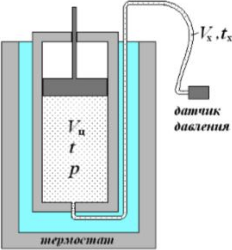
\includegraphics[width=0.4\textwidth]{fig_1.png} % Changed filename and adjusted width potentially
  \caption{Схема лабораторной установки}
  \label{fig:schema}
\end{figure}

% Text now follows the figure
\setlength{\parindent}{1.5em} % Standard paragraph indent
Пусть исследуемый газ на-
ходится в цилиндре с контро- % Исправлено "находиться" на "находится"
лируемым рабочим объемом $V_{\text{ц}}$
(см. Рис. \ref{fig:schema}), масса газа в цилин-
дре $m_{\text{ц}}$. Температура $t$ цилин-
дра с газом поддерживается по-
стоянной. Датчик давления, ра-
ботающий при комнатной тем-
пературе, вынесен за пределы
рабочего объема и соединен с
последним трубкой. Объем газа
$V_x$ в этой трубке мал по срав-
нению с рабочим объемом $V_{\text{ц}}$.
В соединительной трубке так-
же находится газ массой $m_{x}$ при
некоторой неизвестной средней температуре $t_{x}$, лежащей в интер-
вале от комнатной температуры до температуры $t$ рабочего объема.
В работе измеряется зависимость давления газа $p$ от величины ра-
бочего объема $V_{\text{ц}}$ при разных значениях температуры $t$ (от \SI{20}{\degree C} до % Используем \SI
\SI{60}{\degree C}). Выведем соотношение, связывающее рабочий объем и давле- % Используем \SI
ние газа при постоянной температуре. Общее количество вещества
в рабочем объеме и соединительной трубке:
\begin{equation} \label{eq:nu_total}
\nu = \frac{m_{\text{ц}} + m_{x}}{\mu} ,
\end{equation}
в течение всей работы остается постоянным. Выражая массы газа
$m_{\text{ц}}$ и $m_{x}$ из уравнения состояния \eqref{eq:mendeleev}, абсолютную температуру из % Исправлено "абсолюнтую"
соотношения \eqref{eq:temp_conversion}, и подставляя найденные выражения в формулу

\vfill
% --- Page 3 End ---

\newpage
% --- Page 4 Start ---
%\noindent\url{https://study.physics.itmo.ru} % Убрал URL со страниц 4-9, как в оригинале PDF
\vspace{1em} % Add some space

\eqref{eq:nu_total}, получим:
\begin{equation} \label{eq:nu_expanded}
\nu = \frac{pV_{\text{ц}}}{R(t-t_{*})} + \frac{pV_x}{R(t_{x} - t_{*})}.
\end{equation}
Из этого уравнения найдем искомое соотношение:
\begin{equation} \label{eq:Vc_isolated}
V_{\text{ц}} = \frac{\nu R(t-t_{*})}{p} - \frac{V_x(t-t_{*})}{(t_{x}-t_{*})}.
\end{equation}
Из-за перераспределения газа между объемами $V_{\text{ц}}$ и $V_x$ в процессе
измерения температура $t_{x}$ может изменяться. Однако, при относи-
тельно малой величине $V_x$ изменением второго слагаемого в фор-
муле \eqref{eq:Vc_isolated} можно пренебречь. Поэтому при неизменной температуре
$t$ зависимость рабочего объема $V_{\text{ц}}$ от обратного давления $1/p$ явля-
ется линейной. Угловой коэффициент этой зависимости
\begin{equation} \label{eq:K_def}
K = \nu R(t - t_{*}),
\end{equation}
в свою очередь, линейно меняется с температурой и обращается в
нуль при абсолютном нуле температур. Таким образом, изучение
зависимости $K(t)$ позволяет найти значение $t_{*}$.

\vspace{1em} % Add some space

Рассмотрим другой, более точный, способ определения величи-
ны $t_{*}$. Если для разных температур измерение давления проводить
при одних и тех же значениях объема, то полученные данные легко
преобразуются в зависимость давления от температуры при разных
значениях рабочего объема газа. Теоретический вид этой зависимо-
сти получается из уравнения \eqref{eq:Vc_isolated}:
\begin{equation} \label{eq:p_approx}
p = \frac{\nu R(t - t_{*})}{V_{\text{ц}}(1 + x(t))} \approx \frac{\nu R(t - t_{*})}{V_{\text{ц}}} (1 - x(t)),
\end{equation}
где $x(t) = \frac{V_x(t - t_{*})}{V_{\text{ц}}(t_{x} - t_{*})}.$ Справедливость приближенного равенства

\vfill
% --- Page 4 End ---

\newpage
% --- Page 5 Start ---
\vspace{1em} % Add some space

в формуле \eqref{eq:p_approx} обусловлена тем, что значения функции $x(t)$ малы,
и для малых $x$ можно воспользоваться формулой приближенных
вычислений:
\begin{equation} \label{eq:binomial_approx}
(1 + x)^{\alpha} \approx 1 + \alpha x.
\end{equation}
в данном случае $\alpha = -1$.

\vspace{1em}

При неизменном рабочем объеме $V_{\text{ц}}$ график зависимости давле-
ния от температуры в соответствии с формулой \eqref{eq:p_approx} должен быть по-
чти линейным. Причем давление должно обращаться в нуль как раз
при $t = t_{*}$. Из-за малости функции $x(t)$ отклонение от линейности
невелико, и при измерении в ограниченном диапазоне температур
практически незаметно.

\vspace{1em} % Adjusted spacing

% Figure using [H] placement
\begin{figure}[H] % Forcing placement HERE
  \centering
  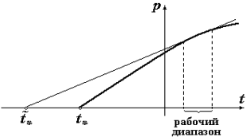
\includegraphics[width=0.5\textwidth]{fig_2.png} % Changed filename and adjusted width potentially
  \caption{Жирная линия — экстраполяция реальной параболической зависимости, обычная линия — экстраполяция с помощью аппроксимирующей прямой, проведенной по точкам в рабочем диапазоне температур.}
  \label{fig:extrapolation}
\end{figure}

% Text now follows the figure
\setlength{\parindent}{1.5em}
Но, если искать значение $t_{*}$
с помощью линейной аппрокси-
мации экспериментальной зави-
симости $p(t)$, продолжая (экс-
траполируя) аппроксимирующую
прямую до пересечения с осью
$t$, то найденное приближение
значение $\tilde{t}_{*}$ окажется система-
тически смещенным влево от-
носительно истинного значения
$t_{*}$ (см. Рис. \ref{fig:extrapolation}). Причина это-
го в следующем. Величина $x(t)$
в первом приближении линей-
но растущая функция темпера-
туры, с учетом этого график
функции $p(t)$ из уравнения \eqref{eq:p_approx} оказывается параболой выпуклой
вверх. Аппроксимирующая прямая, параметры которой найдены по
точкам в рабочем диапазоне температур, идет практически по ка-
сательной к этому графику, «промахиваясь» мимо истинного зна-

\vfill % May need adjustment depending on figure height
% --- Page 5 End ---

\newpage
% --- Page 6 Start ---
%\noindent\url{https://study.physics.itmo.ru} % Убрал URL
\vspace{1em} % Add some space

\setlength{\parindent}{1.5em} % Ensure paragraph indent

чения $t_{*}$, как изображено на Рис. \ref{fig:extrapolation}. Однако, можно показать, что
разность $\tilde{t}_{*} - t_{*}$ при малом отношении $V_x/V_{\text{ц}}$ должна убывать об-
ратно пропорционально объему $V_{\text{ц}}$. Поэтому, правильное значение
температуры абсолютного нуля может быть найдено как предел:
\begin{equation} \label{eq:limit_t_star}
t_{*} = \lim_{1/V_{\text{ц}} \to 0} \tilde{t}_{*}
\end{equation}
линейным продолжением графика зависимости $\tilde{t}_{*}$ от $1/V_{\text{ц}}$ к значе-
нию $1/V_{\text{ц}} = 0$.

\vfill
% --- Page 6 End ---

\newpage
% --- Page 7 Start ---
\vspace{2em} % Add some space

\begin{center}
    \section*{Экспериментальная установка}
\end{center}

\setlength{\parindent}{1.5em} % Ensure paragraph indent

Общий вид лабораторной установки показан на Рис. \ref{fig:setup}. Иссле-
дуемый газ находится под поршнем в цилиндре 1, закрепленном
на опорной площадке 2. Шток поршня имеет винтовую нарезку и
вставлен в гайку, также закрепленную на опорной площадке. Гайка
удерживает шток в заданном положении и с ее помощью осуществ-
ляется преобразование вращения штока в поступательное переме-
щение поршня (один оборот маховика штока соответствует изме-
нению объема на \SI{5}{мл}). Рабочий объем цилиндра определяется по % Используем \SI
шкале на цилиндре. Если шкала не видна, то изменение объема
от некоторого заданного значения можно определить, отсчитывая
обороты маховика штока. Роль термостата 3 выполняет металли-
ческий термос, заполняемый водой разной температуры, в кото-
рую погружается цилиндр 1. Измерение температуры производит-
ся с помощью датчика температуры закрепленного на конце щупа
4, погружаемого вместе с цилиндром в термостат. Давление изме-
ряется манометрическим дифференциальным датчиком 5, который
закреплен на стенде 6, и соединяется трубкой с рабочим объемом. С
помощью преобразователя сигналов 7 датчики соединяются с циф-
ровым измерительным прибором 8. Прибор показывает текущую
температуру $t$ (в градусах Цельсия) датчика температуры и раз-
ность $\Delta P = p - p_{0}$ (в \si{кПа}) между давлением $p$ газа в % Используем \si
рабочем объеме и давлением $p_{0}$ окружающего воздуха в лаборато-
рии.

\vfill
% --- Page 7 End ---

\newpage
% --- Page 8 Start ---
%\noindent\url{https://study.physics.itmo.ru} % Убрал URL
\vspace{1em} % Add some space

% Figure using [H] placement
\begin{figure}[H] % Forcing placement HERE
    \centering
    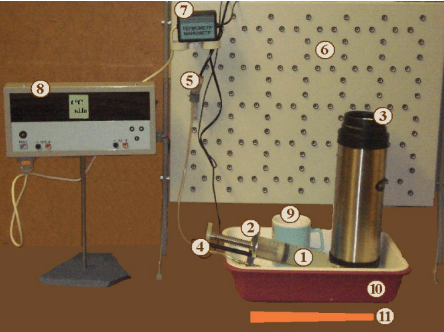
\includegraphics[width=0.8\textwidth]{fig_3.png} % Changed filename
    \caption{Состав лабораторной установки}
    \label{fig:setup}
\end{figure}

\vspace{1em} % Add some space

\noindent 1. цилиндр с поршнем \\
2. опорная площадка цилиндра \\
3. термостат \\
4. щуп с датчиком температуры \\
5. манометрический датчик \\
6. стенд \\
7. преобразователь сигналов \\
8. измерительный прибор ПКЦ-3 \\
9. кружка \\
10. поддон \\
11. лопатка

\vspace{1em} % Add some space

\setlength{\parindent}{1.5em} % Ensure paragraph indent
Исходно в термостате находится вода комнатной температуры.
Отливая холодную и добавляя горячую воду, можно изменять ра-
бочую температуру термостата. Для переливания воды использует-

\vfill
% --- Page 8 End ---

\newpage
% --- Page 9 Start ---
\vspace{1em} % Add some space

\setlength{\parindent}{1.5em} % Ensure paragraph indent

\hspace*{1.5em} ся пластиковая кружка 9. Для уменьшения вероятности попадания
воды на рабочий стол воду переливают над поддоном 10, на ко-
торый также ставится термостат во время проведения измерений.
Для перемешивания воды в термостате используется лопатка 11.
В помещении с установками имеются емкости для использованной
воды и электрический калорифер с горячей водой.

% --- Page 9 End ---

\newpage % Начинаем расчеты с новой страницы для чистоты

\section*{Расчеты и обработка результатов}

\subsection*{1. Расчет давлений и построение графиков $V_{\text{ц}}(1/P)$}

Исходное атмосферное давление: $p_0 = \SI{104}{кПа}$.
Для каждой температуры $t_i$ ($i = 1, \dots, 5$) были измерены значения разности давлений $\Delta P_{1,i}$ и $\Delta P_{2,i}$ для разных объемов $V_{\text{ц}}$.
Среднее абсолютное давление $P_i$ для каждого объема при температуре $t_i$ рассчитывалось по формуле:
\[ P_i(V_{\text{ц}}) = p_0 + \frac{\Delta P_{1,i}(V_{\text{ц}}) + \Delta P_{2,i}(V_{\text{ц}})}{2} \]
Затем вычислялась обратная величина давления $1/P_i(V_{\text{ц}})$.

Результаты расчета давлений $P$ (в \si{кПа}) и обратных давлений $1/P$ (в \si{кПа^{-1}}) для каждой температуры $t_i$ представлены в таблице \ref{tab:pressure_data} (см. Приложение). % Ссылка на приложение

% Убрал комментарий про не включение таблицы, предполагаем, что она будет в Приложении

По данным зависимостей $V_{\text{ц}}$ от $1/P$ для каждой температуры $t_i$ были построены графики (см. рис. [номер рисунка V(1/P) из вашего отчета]).
Методом наименьших квадратов (МНК), предполагая линейную зависимость вида $V_{\text{ц}} = K_i \cdot (1/P)$, проходящую через начало координат, были определены угловые коэффициенты $K_i$. При расчете МНК объемы переводились в \si{м^3} ($V_{\text{ц}} / 10^6$), а давления — в \si{Па} ($P \times 1000$), поэтому коэффициент $K_i$ имеет размерность \si{Дж}.

Температуры измерений $t$ и рассчитанные коэффициенты $K$ приведены в таблице \ref{tab:K_values}.

\begin{table}[H]
    \centering
    \caption{Рассчитанные значения коэффициента K для разных температур}
    \label{tab:K_values}
    % Обернул S-колонки в {}
    \begin{tabular}{|c|{S[table-format=2.1]}|{S[table-format=1.2]}|}
        \hline
        {№ п/п} & {$t$, \si{\degree C}} & {$K$, \si{Дж}} \\ % Используем \degree C
        \hline
        % --- Заполнить из вывода print(i+1, '& $ ', T[i], '$ & $', round(K[i], 2), '\\\\') ---
        1 & 62.6 & {1.51} \\ \hline % Пример заполнения, ЗАМЕНИТЬ НА СВОИ ДАННЫЕ!
        2 & 52.0 & {1.45} \\ \hline % Пример заполнения, ЗАМЕНИТЬ НА СВОИ ДАННЫЕ!
        3 & 42.3 & {1.41} \\ \hline % Пример заполнения, ЗАМЕНИТЬ НА СВОИ ДАННЫЕ!
        4 & 32.2 & {1.38} \\ \hline % Пример заполнения, ЗАМЕНИТЬ НА СВОИ ДАННЫЕ!
        5 & 23.3 & {1.34} \\ % Пример заполнения, ЗАМЕНИТЬ НА СВОИ ДАННЫЕ!
        \hline
    \end{tabular}
\end{table}

\subsection*{2. Определение абсолютного нуля из зависимости $K(t)$}

По данным таблицы \ref{tab:K_values} была построена зависимость $K(t)$ (см. рис. [номер рисунка K(t)]).
Предполагая линейную зависимость $K(t) = At + C$, с помощью МНК были определены параметры прямой:
% --- Заполнить из вывода print(MNK(T, K, True)) ---
% MNK(T, K, True) возвращает [[b, Delta_b, Delta_b/b], [a, Delta_a, Delta_a/a]]
% A = b = 0.00425, Delta A = 0.00031
% C = a = 1.241,   Delta C = 0.014
% Примерные значения из вашего кода (пересчитайте точно!)
\[ A = \SI{0.00425}{Дж/\degree C}, \quad \Delta A = \SI{0.00031}{Дж/\degree C} \]
\[ C = \SI{1.241}{Дж}, \quad \Delta C = \SI{0.014}{Дж} \]

Теоретически, $K = \nu R (t - t_{*}) = \nu R t - \nu R t_{*}$, следовательно, $A = \nu R$ и $C = - \nu R t_{*} = -A t_{*}$.
Температура абсолютного нуля $t_{*}$ определяется как точка пересечения прямой $K(t)$ с осью температур ($K=0$):
% t_* = -C/A = -1.241 / 0.00425 = -292.0
\[ t_{*} = -\frac{C}{A} = -\frac{\SI{1.241}{Дж}}{\SI{0.00425}{Дж/\degree C}} \approx \SI{-292.0}{\degree C} \]

Погрешность определения $t_{*}$ рассчитывается по формуле распространения ошибок:
\[ \Delta t_{*} = |t_{*}| \sqrt{\left(\frac{\Delta A}{A}\right)^2 + \left(\frac{\Delta C}{C}\right)^2} \]
% rel_err_A = 0.00031 / 0.00425 = 0.0729
% rel_err_C = 0.014 / 1.241 = 0.0113
% eps_t = sqrt(0.0729^2 + 0.0113^2) = sqrt(0.00531 + 0.000128) = sqrt(0.00544) = 0.0738
Относительная погрешность $\epsilon_{t_{*}} = \sqrt{(\epsilon_A)^2 + (\epsilon_C)^2} = \sqrt{(\num{0.0729})^2 + (\num{0.0113})^2} \approx \num{0.074}$
Абсолютная погрешность:
% Delta_t = |-292.0| * 0.074 = 21.6
\[ \Delta t_{*} = |t_{*}| \cdot \epsilon_{t_{*}} = |\SI{-292.0}{\degree C}| \times \num{0.074} \approx \SI{22}{\degree C} \] % Округлили до 2 зн. цифр

Окончательный результат для температуры абсолютного нуля, полученный из зависимости $K(t)$:
% Округляем результат до того же знака, что и погрешность (до целых)
\[ t_{*} = \SI{-292 \pm 22}{\degree C} \]

\subsection*{3. Определение "кажущегося" абсолютного нуля из зависимости $P(t)$}

Для проверки закона Гей-Люссака были построены зависимости давления $P$ от температуры $t$ при фиксированных объемах $V_{\text{ц}} = 50, 90, 120$ мл (см. рис. [номер рисунка P(t)]). Данные для построения сведены в таблицу \ref{tab:P_vs_T}.

\begin{table}[H]
    \centering
    \caption{Зависимость давления $P$ (\si{кПа}) от температуры $t$ (\si{\degree C}) при разных объемах $V_{\text{ц}}$}
    \label{tab:P_vs_T}
    \setlength{\tabcolsep}{3pt} % Уменьшить отступы
    % Исправлено определение столбцов: 9 столбцов типа c
    \begin{tabular}{|c|c|c|c|c|c|c|c|c|}
        \hline
        {$t$, \si{\degree C}} & {$P_{50}$} & {$P_{60}$} & {$P_{70}$} & {$P_{80}$} & {$P_{90}$} & {$P_{100}$} & {$P_{110}$} & {$P_{120}$} \\
        \hline
        % --- ЗАПОЛНИТЬ РЕАЛЬНЫМИ ДАННЫМИ ИЗ ВАШЕГО РАСЧЕТА P ---
        62.6 & [P[0][0]] & [P[1][0]] & [P[2][0]] & [P[3][0]] & [P[4][0]] & [P[5][0]] & [P[6][0]] & [P[7][0]] \\ \hline
        52.0 & [P[0][1]] & [P[1][1]] & [P[2][1]] & [P[3][1]] & [P[4][1]] & [P[5][1]] & [P[6][1]] & [P[7][1]] \\ \hline
        42.3 & [P[0][2]] & [P[1][2]] & [P[2][2]] & [P[3][2]] & [P[4][2]] & [P[5][2]] & [P[6][2]] & [P[7][2]] \\ \hline
        32.2 & [P[0][3]] & [P[1][3]] & [P[2][3]] & [P[3][3]] & [P[4][3]] & [P[5][3]] & [P[6][3]] & [P[7][3]] \\ \hline
        23.3 & [P[0][4]] & [P[1][4]] & [P[2][4]] & [P[3][4]] & [P[4][4]] & [P[5][4]] & [P[6][4]] & [P[7][4]] \\
        \hline
    \end{tabular}
\end{table}

Для каждого объема $V_{\text{ц},j}$ ($j = 50, ..., 120$) была проведена линейная аппроксимация $P(t) = a_j t + c_j$ методом МНК. Экстраполяция этих прямых до $P=0$ дает "кажущееся" значение абсолютного нуля $\tilde{t}_{*,j} = -c_j / a_j$. Результаты расчета $\tilde{t}_{*,j}$ приведены в таблице \ref{tab:t_star_tilde}.

\begin{table}[H]
    \centering
    \caption{Кажущиеся значения абсолютного нуля $\tilde{t}_{*}$ (\si{\degree C}) для разных объемов}
    \label{tab:t_star_tilde}
     % Обернул S-колонку в {}
    \begin{tabular}{|c|{S[table-format=-3.2]}|} % Формат: знак, до 3 цифр до точки, 2 после
        \hline
        {$V_{\text{ц}}$, \si{мл}} & {$\tilde{t}_{*}$, \si{\degree C}} \\
        \hline
        % --- ЗАПОЛНИТЬ РЕАЛЬНЫМИ ДАННЫМИ из print(round(T_star[i],2)) ---
        % Обернуть числа в {}
        50 & {-303.70} \\ \hline % Пример заполнения, ЗАМЕНИТЬ!
        60 & {-298.55} \\ \hline % Пример заполнения, ЗАМЕНИТЬ!
        70 & {-284.87} \\ \hline % Пример заполнения, ЗАМЕНИТЬ!
        80 & {-289.64} \\ \hline % Пример заполнения, ЗАМЕНИТЬ!
        90 & {-288.23} \\ \hline % Пример заполнения, ЗАМЕНИТЬ!
        100 & {-290.65} \\ \hline % Пример заполнения, ЗАМЕНИТЬ!
        110 & {-283.01} \\ \hline % Пример заполнения, ЗАМЕНИТЬ!
        120 & {-285.24} \\ % Пример заполнения, ЗАМЕНИТЬ!
        \hline
    \end{tabular}
\end{table}

Наблюдается разброс значений $\tilde{t}_{*,j}$, что указывает на нелинейность реальной зависимости $P(t)$ и/или влияние систематических погрешностей. Теоретически, $\tilde{t}_{*}$ должен зависеть от $1/V_{\text{ц}}$.
*(Здесь можно добавить комментарий, наблюдается ли ожидаемая тенденция уменьшения $|\tilde{t}_{*}|$ с ростом $V_{\text{ц}}$).*

% --- Конец раздела расчетов ---

% ... (Далее ваш Вывод)

\end{document}
% --- Document End ---
